\documentclass{beamer}

\usepackage{listings}
\usepackage[T1]{fontenc}
\usepackage{graphicx}
\usepackage[utf8]{inputenc}
\usepackage{xcolor}
\usepackage{amsmath,amssymb}
\usepackage{mathtools}
\usepackage[linesnumbered,lined,boxed,commentsnumbered,ruled,vlined]{algorithm2e}
\usepackage{csquotes}
\usepackage{templates/beamerthemekit}
\usepackage{pgfplots}
\usepackage{xpatch}

\newcommand{\sls}{Safer Language Subset}
\newcommand{\slss}{Safer Language Subsets}

\newcommand{\sqs}{Software-Qualitätsstandard}
\newcommand{\sqss}{Software-Qualitätsstandards}

\newcommand{\misra}{MISRA-C}

\lstset{language=C,
    basicstyle=\ttfamily,
    keywordstyle=\color{blue}\ttfamily,
    stringstyle=\color{red}\ttfamily,
    commentstyle=\color{gray}\ttfamily,
    morecomment=[l][\color{gray}]{\#}
}

\titleimage{Titelbild}

\titlelogo{empty}

\graphicspath{{./graphics/}}%helpful if your graphic files are in another directory

\title{M10: \sqss}
\author[Linder]{Alexander Linder}
\date{20.02.2020}
\institute{FAKULTÄT FÜR INFORMATIK}
%\titlegraphic{\includegraphics[scale=0.1]{title.png}}

\begin{document}
    \setbeamercovered{invisible}
    % change the following line to "ngerman" for German style date and logos
    \selectlanguage{ngerman}

    \begin{frame}
        \maketitle
    \end{frame}

    \begin{frame}
        \tableofcontents
    \end{frame}

    \section{Motivation}
    \label{sec:motivation}
    \begin{frame}{Motivation von \sqss}
        \begin{itemize}
            \item Beschränkung auf sichere Features von Programmiersprachen
            \item Leichtere Wartbarkeit des Codes
            \item Für alle Entwickler einheitliche Richtlinien
            \pause
            \item \textbf{Weniger Programmfehler}
        \end{itemize}
    \end{frame}

    \section{\misra}
    \label{sec:misra-c}
    \begin{frame}{Über \misra}
        \begin{itemize}
            \item Entwickelt durch die \textbf{M}otor \textbf{I}ndustry \textbf{S}oftware \textbf{R}eliability \textbf{A}ssociation
            \item Erste Veröffentlichung 1998
            \item Aktuelle Version von 2012
            \item Verwendbarkeit von C in sicherheitskritischen Anwendungen als primäres Ziel
            \item Präzisiert Unklarheiten im C-Standard
        \end{itemize}
    \end{frame}

    \begin{frame}{Regelsatz 1998 vs 2004}
        \begin{center}
            \begin{tikzpicture}[scale=0.7]
    \pie[sum=auto]{93/ , 34/ }
    \pie[pos={8,0},sum=auto, text=legend]{122/verpflichtend, 20/empfohlen}
\end{tikzpicture}
        \end{center}
    \end{frame}

    \begin{frame}[fragile]{Beispielregel}
        \begin{exampleblock}{Rule 2.1 (required): Assembly language shall be encapsulated and isolated}
            Where assembly language instructions are required it is recommended that they be encapsulated
            and isolated in either (a) assembler functions, (b) C functions or (c) macros.\\
            For reasons of efficiency it is sometimes necessary to embed simple assembly language instructions
            in-line, for example to enable and disable interrupts.
            If it is necessary to do this for any reason, then it is recommended that it be achieved by using macros.\\
            Note that the use of in-line assembly language is an extension to standard C, and therefore also
            requires a deviation against Rule 1.1.
            \begin{lstlisting}[language=C]
                #define NOP asm(" NOP")
            \end{lstlisting}
        \end{exampleblock}
    \end{frame}

    \section{Regelklassifizierung}
    \label{sec:regelklassifizierung}
    \begin{frame}{Motivation}
        \textit{Warum} klassifizieren wir Regeln?
        \pause
        \begin{itemize}
            \item Unterscheidung in \textit{stilistisch} und \textit{funktional} basierte Regeln
            \item Feststellung ihrer \enquote{Güte}
            \item Formale Definition eines \slss
        \end{itemize}
        \pause
        \begin{block}{Güteabstufung}
            \quad \quad Stilistische Regeln\\
            {\boldmath $<$} \quad Rein subjektive, funktionale Regeln\\
            {\boldmath $<$} \quad Empirisch fundierte, funktionale Regeln
        \end{block}
    \end{frame}

    \subsection{Typ A Regeln}
    \label{subsec:typ-a-regeln}
    \begin{frame}{\enquote{Style}-Regeln}
        \only<1-2> {
            \begin{block}{Definition}
                Eine Typ A Regel sei eine Regel, welche alleinig den Stil des Codes beeinflusst.
            \end{block}
            \pause
            \begin{exampleblock}{Rule 5.7 (advisory)}
                No identifier name should be reused.
            \end{exampleblock}
        }
        \only<3> {
            \begin{exampleblock}{Rule 5.7 (advisory)}
                \lstinputlisting{graphics/typa.c}
            \end{exampleblock}
        }
    \end{frame}

    \subsection{Typ B.1 Regeln}
    \label{subsec:typ-b-1-regeln}
    \begin{frame}{Subjektive Regeln}
        \only<1-2> {
            \begin{block}{Definition}
                Eine Typ B.1 Regel sei eine Regel, welche potentiell unsichere Sprachfeatures ausschließt,
                jedoch keine empirischen Daten besitzt, die diesen Ausschluss begründen.
            \end{block}
            \pause
            \begin{exampleblock}{Rule 14.4 (required)}
                The \textit{goto} statement shall not be used.
            \end{exampleblock}
        }
        \only<3> {
            \begin{exampleblock}{Rule 14.4 (required)}
                \lstinputlisting{graphics/typb1.c}
            \end{exampleblock}
        }
    \end{frame}

    \subsection{Typ B.2 Regeln}
    \label{subsec:typ-b-2-regeln}
    \begin{frame}{Evidenzbasierte Regeln}
        \only<1-2> {
            \begin{block}{Definition}
                Eine Typ B.2 Regel sei eine Regel, welche potentiell unsichere Sprachfeatures ausschließt und empirische
                Daten besitzt, die diesen Ausschluss begründen.
            \end{block}
            \pause
            \begin{exampleblock}{Rule 9.1 (required)}
                All automatic variables shall have been asigned a value before being used.
            \end{exampleblock}
        }
        \only<3> {
            \begin{exampleblock}{Rule 9.1 (required)}
                \lstinputlisting{graphics/typb2.c}
            \end{exampleblock}
        }
    \end{frame}

    \section{Safer Language Subsets}
    \label{sec:safer-language-subsets}
    \begin{frame}{Definition}
        \begin{block}{Ein Regelsatz $R$ sei ein \sls $\iff$}
            \begin{itemize}
                \item $R$ enthält nur Typ B.2 Regeln als verpflichtende Regeln
                \item $R$ enthält nur Typ B.1 Regeln als empfohlene Regeln
                \item $R$ enthält keinerlei Typ A Regeln
            \end{itemize}
        \end{block}
        \pause
        $\implies$ $R$ erzwingt nur Regeln, für die es \textit{Evidenz} gibt\\
        \pause
        $\implies$ Regeln in $R$ können aufsteigen, sobald für sie Evidenz gefunden wird
    \end{frame}

    \begin{frame}{Gütekriterien}
        \begin{itemize}
            %\item \only<1>{Regelorthogonalität}\only<2>{\textbf{Regelorthogonalität}}
            \item Orthogonalität
            \item Entscheidbarkeit
            \item Atomizität
            \item Gewichtung
            \item \only<1>{Signal-Rausch-Verhältnis}\only<2>{\textbf{Signal-Rausch-Verhältnis}}
        \end{itemize}
    \end{frame}

    %\begin{frame}{Regelorthogonalität}
    %    \begin{center}
    %        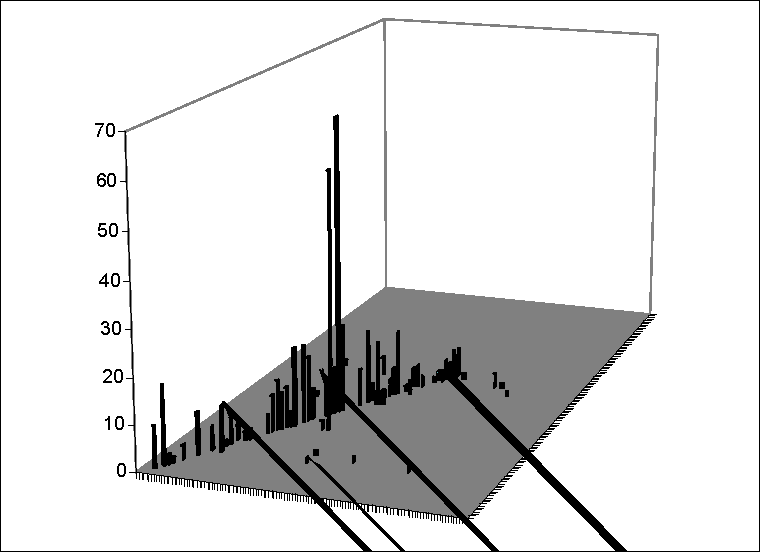
\includegraphics[width=\textwidth,height=0.7\textheight,keepaspectratio]{graphics/rule-crosstalk.pdf}\\
    %        X: Regeln, Y: Dateien mit Tests, Z: Anzahl Tests
    %    \end{center}
    %\end{frame}

    \begin{frame}{Signal-Rausch-Verhältnis}
        \begin{center}
            \begin{overprint}
                \only<1> {
                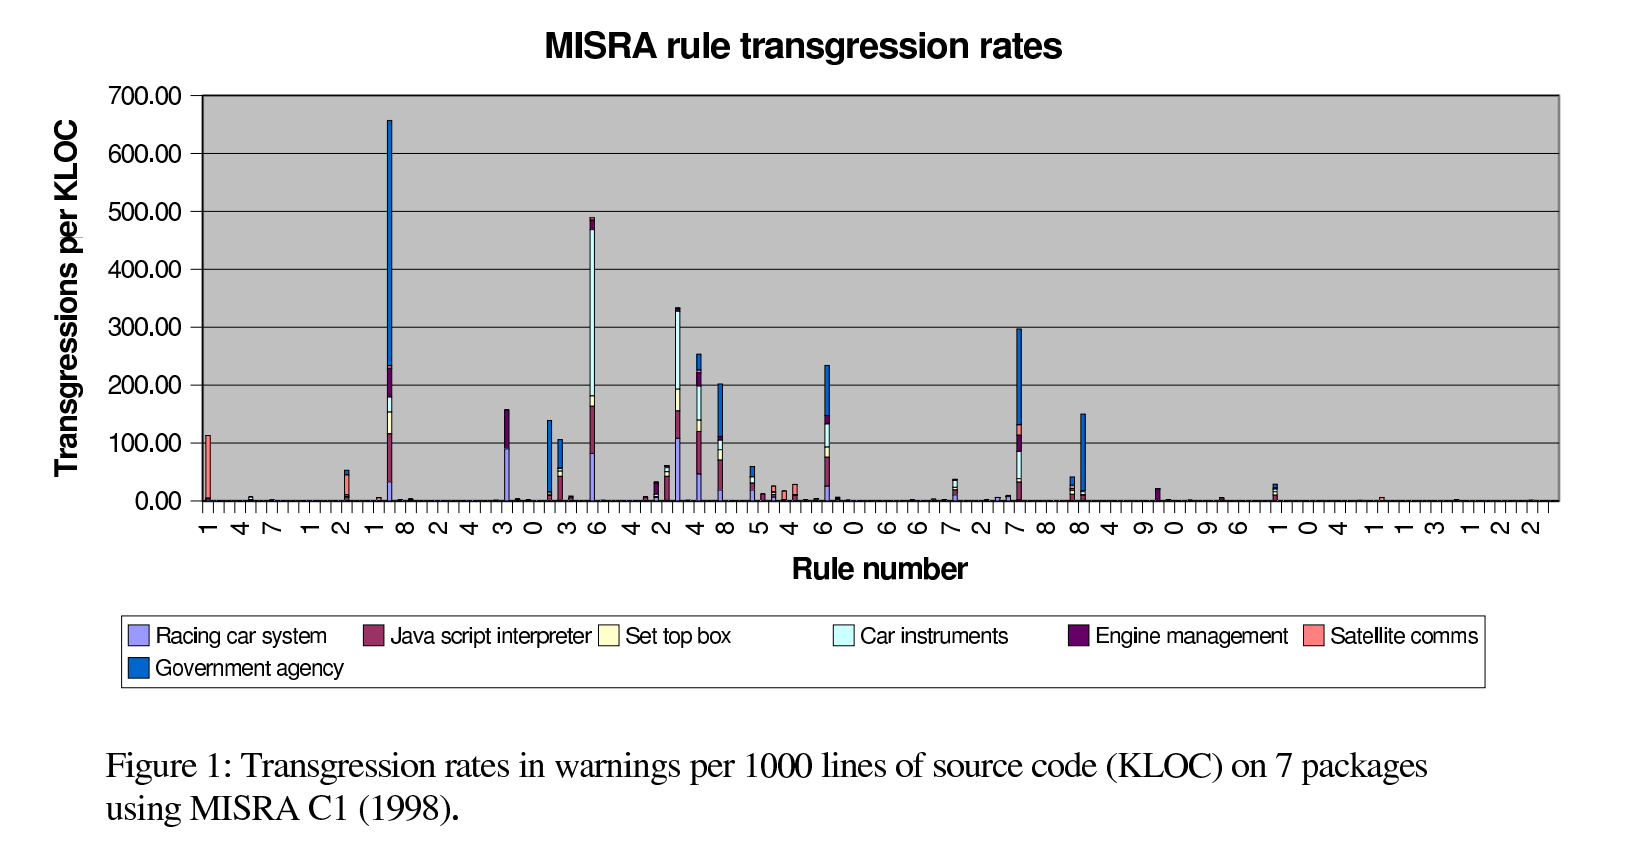
\includegraphics[width=\textwidth,height=0.8\textheight,keepaspectratio]{graphics/1998-transgression-rates.png}
                Verstöße in Warnungen je 1000 Codezeilen auf 7 Pakete verteilt, M1998.
                }
                \only<2> {
                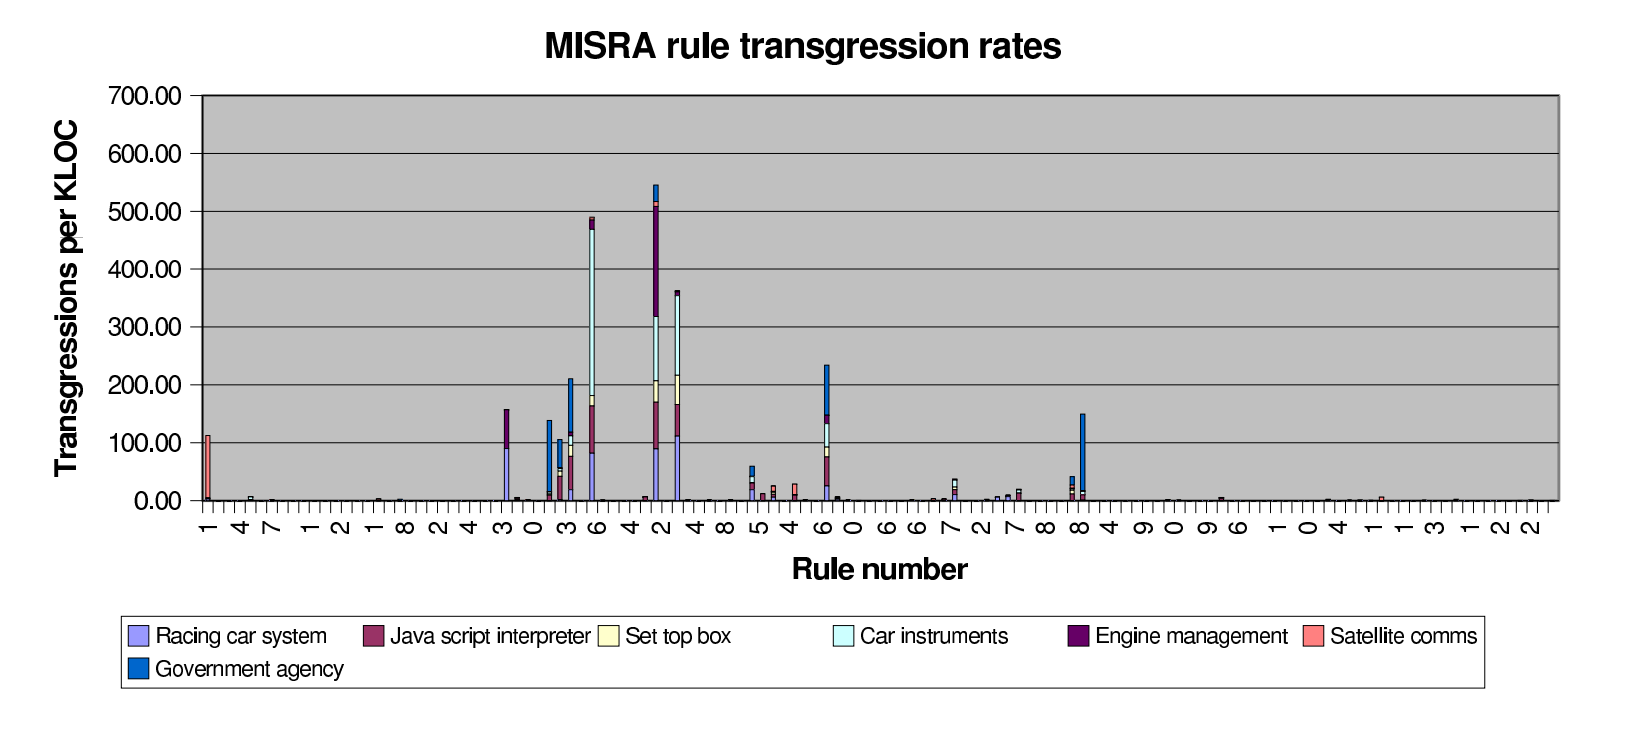
\includegraphics[width=\textwidth,height=0.8\textheight,keepaspectratio]{graphics/2004-transgression-rates.png}
                Verstöße in Warnungen je 1000 Codezeilen auf 7 Pakete verteilt, M2004.
                }
            \end{overprint}
        \end{center}
    \end{frame}

    \section{Fazit}

    \label{sec:fazit}
    \begin{frame}{Fazit}
        \misra\ hat / ist\ldots
        \begin{itemize}
            \item[\ldots] viele gute Regeln
            \item[\ldots] weit verbreitet\\
                $\implies$ tendenziell eher bekannt
            \item[\ldots] wortreiche / unklare Regeln
            \item[\ldots] schlecht entscheidbare Regeln
            \item[\ldots] zu hohes Rauschen in einigen Regeln
        \end{itemize}
        \vspace{0.3cm}
        \pause
        $\implies$ \textbf{Subsets} von \misra\ durchaus brauchbar
    \end{frame}

\end{document}